%%==================================================
%% chapter02.tex for TJU Master Thesis
%% based on CASthesis
%% modified by wei.jianwen@gmail.com
%% Encoding: UTF-8
%%==================================================

\chapter{软管组件理论发展综述}
\section{软管组件概述}
\subsection{软管组件结构}
软管组件,承压能力相对较强,远超普通胶管;结构如图\ref{fig:hose structure}所示,


\begin{figure}[!htbp]
	\centering
	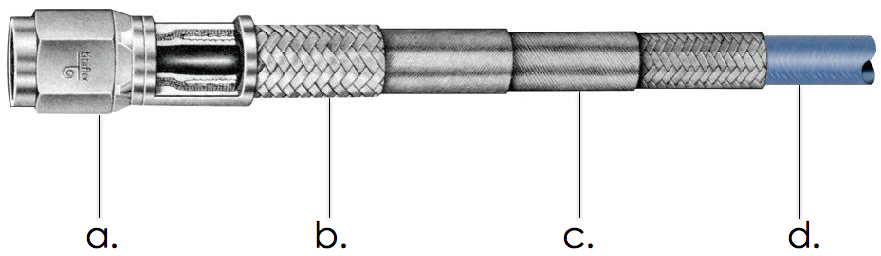
\includegraphics[width=0.6\linewidth]{figure/chap1/Hose-Structure}
	\bicaption[fig:hose structure]{软管组件结构}{软管组件结构(a.接头,b.金属纤维编织层,c.金属纤维缠绕层,d.内管)}{Fig}{Hose Structure(a.Coupling,b.Braid Layer,c.Helix-wound Layer,d.Inner Tube)}
	\label{fig:hose structure}
\end{figure}

\begin{figure}[!htbp]
	\centering
	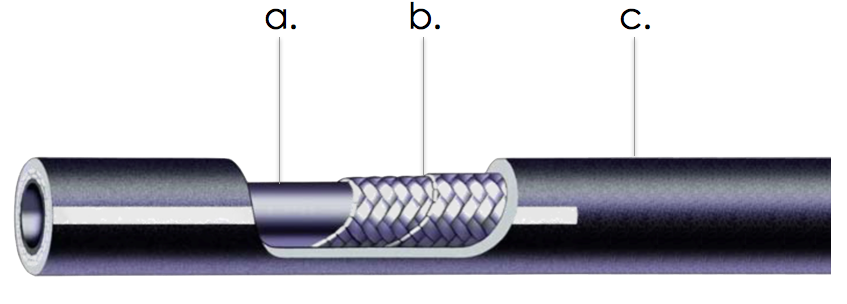
\includegraphics[width=0.6\linewidth]{figure/chap1/Parker-hose}
	\bicaption[fig:hose structure]{软管组件结构}{软管组件结构(a.内管,b.金属纤维编织层,c.保护套)}{Fig}{Hose Structure(a.Inner Tube ,b.Braid Layer,c.Coat Tube)}
	\label{fig:hose structure}
\end{figure}

\subsection{软管组件的生产工艺}

\subsection{软管组件的重要参数}

\section{软管组件的理论发展}


目前对金属编织加强软管的研究,多见于汽车工业中的中刹车管[2]、转向传动管[3]、空调管[4] 等。对软管加强层理论的研究,基本使用通过加强层的总体的要是通过软管理论主要有两个分支[5]:一种是加强层含量较低,橡胶管起主要作用的软管,由Kuipers等人[6,7]提出并完善,适用于帘线加强的软管;另一种是编织加强层主要承力的软管,主要研究的是钢丝螺旋缠绕加强层。软管轴向受拉时,缠绕的金属丝会沿缠绕方向“流动”。编织加强层仅作为螺旋缠绕的一种特例:两层缠绕方向相反,且不允许“流动”的缠绕层[5]。
近20年对编织加强结构的研究主要集中在复合材料编织。复合材料纤维编织的与金属纤维编织的传力机制差别非常明[8]:复合材料纤维只承受单向应力;而金属编织层中的金属丝间的接触关系会直接影响编织层整体的传力,不能忽视。因此,并没有至今尚没有成熟、独立,考虑金属丝间接触关系的编织加强层理论。
有学者尝试用连续介质力学的基本理论推导编织层的本构,如Evans[5]编织层金属纤维侧向传力机制,Horgan等人[9] 提出了纤维加强材料的应变能密度函数,国内学者计算了编织结构强度与突加荷载的情况[10,11]。但主流的研究办法还是结合实验,提出能够反映加强层力学行为的有限元模型。Wijaya[4]对包含软管各层材料及编织层的试件进行了压缩实验,认为金属编织层的应力应变关系是线性的,在软管整体动态特性的研究中取得了较好的效果。Cho[3]研究了编织层在扣压安装接头中的力学行为,结合压缩实验提出了弹塑性的本构模型,Rattensperger[8]同样针对压缩的过程,编织层厚度方向引入一组等效非线性弹簧,表征金属纤维间相互作用。
Hachemi[12]对编织层进行了拉伸试验,将复合材料编织中考虑材料非线性行为的特征单元法(首先由Reese[13]提出)引入金属编织层的研究,提出了能够反映编织结构编织角变化的本构模型。该模型将编织层简化两层Rebar单元,只在编织方向上有刚度。但该模型仍然没有考虑两层Rebar单元之间相互接触的关系。
本研究实验表明,Hachemi[12]本构模型的非线性行为并不足够强,不能与本研究中的高压金属编织加强软管的拉伸实验结果相吻合。我们试图通过引入金属纤维间的接触关系来修正该理论与实验的差距。使得包括非线性段的实验结果都能够与修正后的理论值相吻合。

本研究实验表明,Hachemi[12]本构模型的非线性行为并不足够强,不能与本研究中的高压金属编织加强软管的拉伸实验结果相吻合。我们试图通过引入金属纤维间的接触关系来修正该理论与实验的差距。使得包括非线性段的实验结果都能够与修正后的理论值相吻合。

3.1  引言
特征元法是随着符合材料发展起来的一种方法。这种方法体现的是一种平均化的力学简化思想。将复杂的微观结构转化为一种在小范围内平均等效的力学模型。在材料细观结构与宏观性能之间关系建立起联系是这一系列理论的出发点。长期的探索,特别是近20年来,取得了许多研究成果,并逐渐形成了细观力学这一学科分支。特征元用于力学性能预报与材料优化设计等方面。
特征元法一般在复合材料力学的邻域内比较常见。而对于金属编织层,同样适用,因为特征元并不区分纤维。但仍需要注意以下问题:
	金属纤维与复合材料常用的非金属纤维特性不同:
	金属编织层没有基体,结构易变性大于复合材料;
	编织(Braid)与纺织(Weave)虽然特征元非常类似,但前者为管状结构,后者为平面结构,编织结构的特征元需要考虑额外的约束
3.2  平面编织复合材料的线性与非线性分析
平面编织复合材料的增强相是二向(2D) 织物,其特性以相邻纤维束的间距、纤维束尺寸、每个方向上纤维束的百分含量、纤维束的填充效率和交织线型的复杂程度来表征,虽然编织物的几何形状可作多种改进,但织物结构的内在强度取决于二维平面织物层间的粘结强度。编织结构复合材料的宏观性能主要取决于纤维的编织构造,纤维束与基体材料的类型,纤维束与基体之间界面的损伤等因素。
根据复合材料的构成方式和组分材料的性质,用细观力学的分析方法从理论上估算它的性能,是复合材料研究与开发的一个重要手段[ 2 ]。对于平面织物复合材料,由于在织物中纤维束纵横交错形成波纹状,引起复合材料在织物面内和面外的耦合变形,从而对复合材料的宏观性能产生了重要的影响。T. Ishikawa 及T. W. Chou等人 [3~8] 曾发表过一系列论文研究非混杂织物复合材料的弹性性质分析,他们考虑一个镶嵌模型,采用均匀应力和均匀应变的假定,导出织物复合材料弹性模量的上、下限解。把经典的层合板理论与一维波纹模型结合起来,求平均刚度系数。最近,Lee 等人[ 9 ]提出了一个欧拉伯努利梁模型,来估算带波纹的分段各向同性复合材料的等效弹性模量。张元冲和J . Harding等人[ 10~12 ]利用应变能等效的原理,通过有限元计算,结合平面织物复合材料的单向波纹模型,分析了该类材料的弹性性质。并且在此基础上,根据经典层合板理论,对平面织物复合材料单向波纹模型的上下表面施加不同的约束条件,得出层板弹性常数的变化范围,用有限元能量方法预测出不同铺层数的编织复合材料层板的弹性性能。N. F. Dow 等人 [13] 对织物增强复合材料进行了理论分析及有限元计算。J. H. Byun及T. W. Chou [14] 对平面织物及三维织物复合材料的分析模型做了一个全面的综述。
3.3  镶嵌模型(Mosaic Model)
实际平面织物横断面的纤维束分布如图 2(a)所示,参与编织的纤维束的几何分布非常清晰,经过浸渍基体材料、加压成形后成为波纹状,如图 2 (b)所示,如果忽略波纹状纤维束的连续性,可以将其理想化成镶嵌模型如图 2 (c)所示。如此模型化后,可以将织布增强复合材料看作是二层正交层合板的集合体所组成。图 2 (d)是缎数为8的缎纹平面增强复合材料的模型示意图。镶嵌模型对于缎数较大的混杂平面织物复合材料的弹性系数的初步推定比较适用。
 
图 2镶嵌模型
3.4  正弦波纹模型(Crimp Model)
Ishikawa 等人提出了考虑纤维束弯曲的一维波纹模型,该模型的理论基础同样基于经典层合板理论。描述纤维束弯曲状的一维波纹模型如图2所示。弯曲纤维束的波纹形状用定义于长度为au的区间内函数h1(x) 来表示,与波纹状纤维束相垂直的经向纤维束的透镜形横断面形状用函数h2(x) 来表示。
 
图 3正弦波纹模型
3.5  架桥模型(Bridging Model)
上述波纹模型考虑了纤维束的波纹效果,然而对于被航空部门广泛使用的缎纹织布(SatinWeave)复合材料来说,预报结果低于已知的实验结果。实际上,对于这类复合材料其局部刚度沿两个方向均有所变化,但在一维波纹模型中,仅侧重于受力方向局部刚度的变化。为了克服这一不足,架桥模型考虑了两个方向刚度的变化。在纤维束弯折的编织区域,其局部刚性相对较低,对于缎纹复合材料,网目孤立地配置在代表性单胞中,被周围的直线型纤维束所包围。其周围的层合板部分将分担更多的载荷。以ng =8缎纹织布复合材料为例,架桥模型示意图如图3所示。图3(a)为实际的可重复的最小代表性区域,为六角形。为使模型简单,用等面积的正方形置换六角形区域,如图 4(b)所示。图 4 (c)为该模型各部分之间相互关系的示意图。
 
图 4架桥模型
此模型适用于缎数较高的缎纹织布复合材料,利用架桥模型对缎数为8的碳/ 环氧织布复合材料进行了分析,所得结果与实验结果吻合较好。
3.6  建立在直波纹模型基础上的有限元分析
对于单层平面织物复合材料,张元冲和J .Harding建立了单向直波纹模型,假设平面织物复合材料单层具有宏观正交各向异性的弹性性质,并以经向、纬向和与织物面垂直的法线为它的3个材料主轴,然后利用应变能等效的原理,采用数值细观力学的分析方法,通过有限元计算,分析了平面织物复合材料的机械性能。其单向波纹模型和代表性单胞如图4所示。
 
图 5直波纹模型
对于单层平面编织复合材料层板,张元冲通过对以上模型的上下表面施加不同的约束条件,即想象在层合板中,各个单层所处的状态由于其位置的不同,单层的上下表面约束状态是不一样的,因而对整个层板弹性性质的贡献也是不同的,从而层板的弹性性质随层数变化。但可以用一个单层板处于局部翘曲变形完全受到约束和局部翘曲变形完全自由两种极状态来表征这种变化范围。一般而言,在层板中各个单层所处的状态总是介于上述极限状态中间。而整个层板所表现出的宏观弹性性质,则是各个单层性质的某种平均,因此可以期望由上述两种情况所预测的宏观性质给出层板弹性性质的变化范围。在以上研究基础上,张元冲根据经典层合板理论,得出层板弹性常数的变化范围,用有限元能量方法则预测出不同铺层数的编织复合材料层板的弹性性能。
3.7  结构力学的刚架模型
横山敦土及前川善一郎等人发表一系列论文[ 15~19 ],从结构力学的观点出发,注重编织复合材料内各组分材料、以及交叉纤维束之间的相互作用,采用由梁单元组成的结构模拟平面织物增强复合材料,利用二维有限元法对单胞的力学响应进行分析,其模型如图5所示。
 
图 6结构力学刚架模型
材料单胞的结构力学模型由基体材料梁元和纤维束梁元组成,,在分析中充分考虑纤维束的形态,在纤维束之间的交叉点设置了反映基体作用的由基体材料形成的梁单元,基体与基体之间的相互作用也用基体梁单元进行模拟,其交叉纤维束处的结构力学模型如图5所示。梁单元选用矩形截面形状,其截面尺寸根据对复合材料的显微镜观察来确定。对于平面织物复合材料薄板试件来说,由于处于边缘部位和中央部位织物具有不同的结构,选取不同的结构单胞模型进行分析得出其局部的材料性能。在求得试件局部材料性能后,再进一步利用二维有限元对试件进行分析,得出试件的力学响应。作者试图利用该模型对该类复合材料进行强度预报,然而该模型在实际应用中存在一系列问题,诸如,在模型中各类梁单元的尺寸及形状、材料性质、梁单元的弯曲刚度等均难于恰当地定量选取,给模型的有效应用带来困难。
3.8  平面织物复合材料的非线性分析
复合材料是一种典型的多相材料,具有明显的细观结构,和传统的金属材料相比其变形有显著的过程性。复合材料弹塑性行为的研究大致按两条路线发展,一条是宏观力学的方法,另一条是细观力学的方法。宏观力学的方法是一种唯象理论,不考虑复合材料的微结构。细观力学的方法是根据组分析料的性质、体积分数和微结构状态,研究复合材料的宏观响应与微结构参数间的关系。细观力学的优点是可以帮助理解复合材料的变形机理,并且能够对复合材料的宏观行为做出预测. C. T. Sun 等人 [20, 21]对单向纤维增强复合材料的非线性行为进行了研究。
Ishikawa[ 5 ]在关于线弹性行为研究取得进展之后,进一步对由复合材料各组成部分所特有的非线性引起的平面织物复合材料宏观非线性行为进行了详细研究。其中包括:
1.	与宏观载荷垂直方向的脆性破坏 —knee效应。与载荷垂直的经纱束区域的破坏应变比其它区域小,因此经纱束区域内应变达到某一值时,即顺次发生失效。失效发生后层板材料的切向刚度下降。实际上,在材料内部的很多区域,出现了微裂纹,产生了极其复杂的应力应变场,尽管如此仍然假设经典层板理论有效。
2.	波纹纤维束的偏轴(Off2axis)效应。引起材料非线性行为的另一原因为平面编织物中波纹纤维束的偏轴效应。在单向纤维增强复合材料中,在剪应力作用下,其非线性行为比较显著。然而,在偏轴状态下,即使仅作用拉伸载荷,材料也将表现出非线性行为。这可以通过引入弹性系数的高阶量来分析。
3.	纯基体区域的非线性. Ishikawa 在前述分析基础上,详细地研究了以上各因素对平面编织复合材料非线性行为的影响,并将分析结果与实验结果、有限元数值分析结果进行了对比。
Yokoyama等人在利用刚架模型对平面织物复合材料板状试样的弹性常数进行分析的基础上,进一步用有限元法对试样的强度与破坏进行了研究,预报了其拉伸强度并对其破坏行为进行了模拟。在刚架模型中,由梁单元组成的结构在外力作用下,其各组成部分承受应力的作用,当此应力达到其强度时即发生破坏。发生破坏的梁单元其刚度下降,然后进一步增加载荷增量,得到宏观的材料非线性行为。
3.9  三维编织复合材料的宏观性能研究
复合材料三维整体编织技术是国外80年代由二维编织技术发展起来的高新纺织技术。当时,人们因研究改善复合材料的抗冲击损伤特性问题,提出了复合材料三维整体结构具有优良的抗冲击损伤性能的观点。这一观点为以后的一系列实验所证实,因而这种新型复合材料倍受重视,三维整体编织技术随之获得迅速发展。
复合材料三维整体编织结构出现的时间不长,关于其力学性能的研究感性多于理性,实验研究多于理论研究。国外对于这种新型结构材料的研究已取得了一些成果。其研究大多对被称作单胞的材料代表性单元进行微观分析,然后利用其分析结果再对结构进行宏观分析。有代表性的研究工作主要有: Whit ney[ 22 ], Yang[ 23 ], Crane[ 24 ]等基于二维层合板理论的分析模型、八田博志[ 25 ]及梁军[ 26 ,27 ]等的等效夹杂法、Ma[ 28 ]的弹性应变能方法、Yang和Chou[ 29 ]的纤维偏斜模型、高野直树[ 30 ]的均匀化方法、吴德隆[ 31 ,32 ]的三细胞模型、Розе和 Жигун[ 33 ]提出的弯曲纤维模型、Креге рс[ 34 ]的刚度平均化方法等,这些研究大多以模量分析为中心,其中文献[ 26 , 27 , 30 ]的分析方法可用于研究损伤对编织复合材料力学性能的影响。文献[ 31 , 32 ]针对以四步法为基础编织复合材料,讨论了材料的双模量、弹塑性本构关系及损伤对力学性能的影响问题。T. W.Chou[ 35 ]在他的专著中系统全面地研究了编织复合材料的力学特性和编织工艺。由于编织复合材料结构的复杂性和多样性,使其损伤和强度的非线性研究较之模量研究成果差之甚大,还有许多工作有待于进一步深入探讨。
随着计算机技术的不断发展,越来越多利用有限元计算编织复合材料宏观性能的方法涌现出来,如D. E. Walrat h及赫晓东[ 36 ,37 ]的有限元法,Whyte的有限几何模型(Finite Geometry Model)[ 38 ]、有限体胞模型(Finite Cell Model)[ 39 ]、离散有限元素模型(Discrete Finite Element Model)[ 40 ]及庞宝君[ 41 ]针对四向编织复合材料弹性模量及损伤研究的细观计算力学方法等,它们的出现为纤维织物的工程设计与优化提供了更加便利的手段。国际上最有影响的复合材料期刊J . Comp. Mat h.和Comp. Sci.  Tech.对编织复合材料方面的论文近几年也有大量报道,有关三维编织复合材料有效性能预报方面的综述和理论专著参见文献 [42 ~45] 。
3. 1 修正基体法(Modified Matrix Method)
研究三维编织复合材料性能的方法最早是由 Тарнополскнй等人[ 46 ]利用平均化的观点提出来的,它仅能讨论相互正交三向直线连续纤维增强复合材料的情况。修正基体法一般将三维复合材料通过修正的基体模型简化成二维结构,然后根据现有的理论计算二维编织材料的弹性模量,所不同的是修正基体的性能是由正交于二维结构平面的纤维和基体组分性能平均化得到。Жигун[ 47 ]实验测试了3D正交GRP材料的弹性模量。后来,人们将修正基体法与弯曲纤维模型结合起来,推广到曲线编织纤维复合材料有效性能的研究中去。
3.10  弯曲纤维模型(Curved Fibers Model)
这个模型首次考虑了弯曲纤维织物对复合材料宏观性能的影响. Розе和 Жигун[ 33 ]根据当时二维纤维编织材料的结构特点,针对弯曲纤维提出如图 7所示的计算模型。
文献中根据编织纤维的几何轨迹,给出了复合材料性能随纤维弯曲角度变化的关系曲线,并与文献[ 48 ]的实验结果进行了比较。Плуме等人[ 49 ]将修正基体法与弯曲纤维模型结合起来,研究了温度场下复合材料的热变形,计算了曲线编织复合材料的热膨胀系数。
 
图 7弯曲纤维的计算模型
3.11  刚度平均化方法(Stiff ness Averaging Method)
1978年 Креге рс[ 34 ]提出了预报空间增强复合材料宏观性能的刚度平均化方法。在方法中假设增强纤维是理想直线的圆截面杆,纤维和基体组分是物理线性和各向同性材料。图7给出了三向正交、细编穿刺、四向及六向编织等复合材料的代表性体胞单元。
 
图 8刚度平均化模型
Креге рс等人[ 50 ]后来又在此基础上做了进一步的研究。文献[ 51 ]还利用逐段积分的方法解决了纤维曲线编织复合材料性能预报的难题,思路上与弯曲纤维模型相近。文献[ 52 , 53 ]根据基体材料的不同性质(弹塑性和粘弹性),分别利用改进的刚度平均法建立各自的力学模型,研究了弹性模量与塑性变形及承载时间历程之间的关系,从而推广了三维编织复合材料有效性能的研究范围。
由于复合材料多种特性(如弹性与热膨胀性质、热传导与导电性质等)在数学上的相似性,Креяе рс等人利用刚度平均法在对编织复合材料弹性性能描述的同时,也对其它特性给予讨论。文献[ 54 ]研究了含孔隙编织复合材料的热传导系数。文献[ 55 ]利用平均化方法导出了编织复合材料热膨胀系数的上下限公式。上述工作综述性文章可参见文献[ 56 ~58 ]。
3.12  纤维偏斜模型(Fiber Inclination Model)
T. W. Chou等学者[ 29 ]以由四步法编织的四向编织复合材料为对象,根据其预件内纤维束的排列为锯齿形的特点,建立了纤维偏斜模型,如图8所示。认为在单胞内纤维束沿长方体的4个对角线方向排列,在注入基体后形成一个薄的斜板,4个偏斜的单向薄板形成一个单元。
 
图 9纤维偏斜模型
该模型的理论基础为经典层板理论,在模型中做如下假定:
1.	复合材料内纤维段均平行于矩形体胞单元的对角线方向,加注基体后形成一个斜板。
2.	在一个斜板内的纤维束被认为是理想化的直线,并且是单向的,纤维在单胞边界处转向引起的弯曲和纤维束之间的相互作用忽略不计。
3.	图8所示的四向编织复合材料单胞被看作是由四个单向斜板的集合组成的,单向斜板之间的相互作用忽略不计。各斜板的方向由斜板内的纤维束方向唯一确定,各斜板的厚度相同,斜板内纤维所占体积分数与整体材料纤维体积分数相同。
3.13  非弹性有限元模型( Inelastic Finite Element Model)
法国的Delneste等人[ 61 ,62 ]建立了非弹性有限元分析模型,该模型以四向编织复合材料为例,将复合材料立方体单胞理想化为由一个各向同性弹塑性材料立方体和一个沿4个纤维束方向具有单轴刚度的正交线弹性材料立方体叠加而成,如图9所示。由此可以建立有限元模型的刚度矩阵,利用有限元法对四向编织复合材料结构件进行分析。
 
图 10非弹性有限元模型
3.14  有限几何模型(Finite Geometry Model)
从材料加工科学的观点来看,三维编织复合材料模型的建立都是从其几何单元的剖析开始的。Whyte等人[ 38 ]根据典型单元几何形状建立了纤维织物的有限几何模型,如图10所示.。这个模型最大特点是它具有处理三向编织和其它多轴方向增强材料(包括五、六和七个方向直的或曲的丝束)的能力。另外,通过材料单元组装的总体刚度矩阵,选择合理的断裂准则,可以预报纤维编织复合材料的应力-应变本构关系和强度。文献[ 38 ]详细说明了有限几何模型的建立过程。
 
图 11有限几何模型
Lei和Ko[ 63 ]利用这个模型分析了三维编织混杂SiC/ Al复合材料的非线性断裂行为,Nilanjan 和Sinha[ 64 ]对多向纤维增强复合材料的热结构进行研究,结果展示了纤维不同取向对热结构参数的影响。




